% Document Type
\documentclass[a4paper,11pt]{article}

% Packages
\usepackage{latexsym}
\usepackage[empty]{fullpage}
\usepackage{titlesec}
\usepackage{marvosym}
\usepackage[usenames,dvipsnames]{color}
\usepackage{verbatim}
\usepackage{enumitem}
\usepackage{fancyhdr}
\usepackage[english]{babel}
\usepackage{tabularx}
\usepackage{graphicx}
\usepackage{color}
\usepackage[table]{xcolor}
% \usepackage{tgbonum}
\usepackage[sfdefault]{ClearSans} %% option 'sfdefault' activates Clear Sans as the default text font
\usepackage[T1]{fontenc}
\usepackage[margin=1.4in]{geometry}
\usepackage{setspace}
\usepackage{multirow}
\usepackage[hidelinks]{hyperref}
\input{glyphtounicode}

% Cover Information
\title{Azryl Shamin bin Azrizal CV}
\author{Azryl Shamin bin Azrizal}
\date{\today}


\pagestyle{fancy}
\fancyhf{} % clear all header and footer fields
\fancyfoot{}
\renewcommand{\headrulewidth}{0pt}
\renewcommand{\footrulewidth}{0pt}


% My Colours
\definecolor{MyBlue}{rgb}{0.17, 0.27, 0.59}
\definecolor{MyBGColor}{rgb}{0.90, 0.94, 0.98}
\definecolor{MyHighlight}{rgb}{1.00, 0.89, 0.00}


% URL
\hypersetup{breaklinks=false,%
% pagecolor=white,%
colorlinks=true,%
linkcolor=MyBlue,%
anchorcolor=MyBlue,%
urlcolor=MyBlue}
\urlstyle{same}


% Adjust margins
\addtolength{\oddsidemargin}{-0.5in}
\addtolength{\evensidemargin}{-0.5in}
\addtolength{\textwidth}{1in}
\addtolength{\topmargin}{-0.7in}
\addtolength{\textheight}{1.0in}

\raggedbottom
\raggedright
\setlength{\tabcolsep}{0in}


% Sections formatting
\titleformat{\section}{
  \vspace{5pt}\raggedright\large\bfseries
}{}{0em}{}[\color{black}\titlerule \vspace{-5pt}]


% Ensure that generate pdf is machine readable/ATS parsable
\pdfgentounicode=1


%-------------------------
% Custom commands
\newcommand{\resumeItem}[2]{
  \item\small{
    {#1}{#2 \vspace{-2pt}}
  }
}


% Just in case someone needs a heading that does not need to be in a list
\newcommand{\resumeHeading}[4]{
    \begin{tabular*}{0.99\textwidth}[t]{l@{\extracolsep{\fill}}r}
      \textbf{#1} & {#2} \\
      \textit{\small#3} & \textit{\footnotesize #4} \\
    \end{tabular*}\vspace{-5pt}
}


\newcommand{\resumeSubheading}[4]{
  \vspace{-1pt}\item
    \begin{tabular*}{0.97\textwidth}[t]{l@{\extracolsep{\fill}}r}
      \textbf{\color{MyBlue} #1} & {\footnotesize#2} \\
      \textit{\footnotesize #3} & \textit{\footnotesize #4} \\
    \end{tabular*}\vspace{-5pt}
}


\newcommand{\resumeSubSubheading}[2]{
    \begin{tabular*}{0.97\textwidth}{l@{\extracolsep{\fill}}r}
      \textit{\footnotesize #1} & \textit{\footnotesize #2} \\
    \end{tabular*}\vspace{-5pt}
}


\newcommand{\resumeSubItem}[2]{\resumeItem{#1}{#2}\vspace{-4pt}}


\renewcommand{\labelitemii}{$\circ$}


\newcommand{\resumeSubHeadingListStart}{\begin{itemize}[leftmargin=*]}
\newcommand{\resumeSubHeadingListEnd}{\end{itemize}}
\newcommand{\resumeItemListStart}{\begin{itemize}}
\newcommand{\resumeItemListEnd}{\end{itemize}\vspace{-5pt}}


% Own symbols
\newcommand{\CC}{C\nolinebreak\hspace{-.05em}\raisebox{.4ex}{\tiny\bf +}\nolinebreak\hspace{-.10em}\raisebox{.4ex}{\tiny\bf +}}
\def\CC{{C\nolinebreak[4]\hspace{-.05em}\raisebox{.4ex}{\tiny\bf ++}}}
\newcommand{\mytextsharp}{$^\sharp$}


%-------------------------------------------
%%%%%%  CV STARTS HERE  %%%%%%%%%%%%%%%%%%%%%%%%%%%%

\begin{document}

%----------HEADING-----------------
\begin{tabular*}{\textwidth\footnotesize}{ll @{\extracolsep{\fill}}r}
  \multirow{5}{*}{
    \begin{minipage}[l][2.0cm][c]{2.25cm}
    % 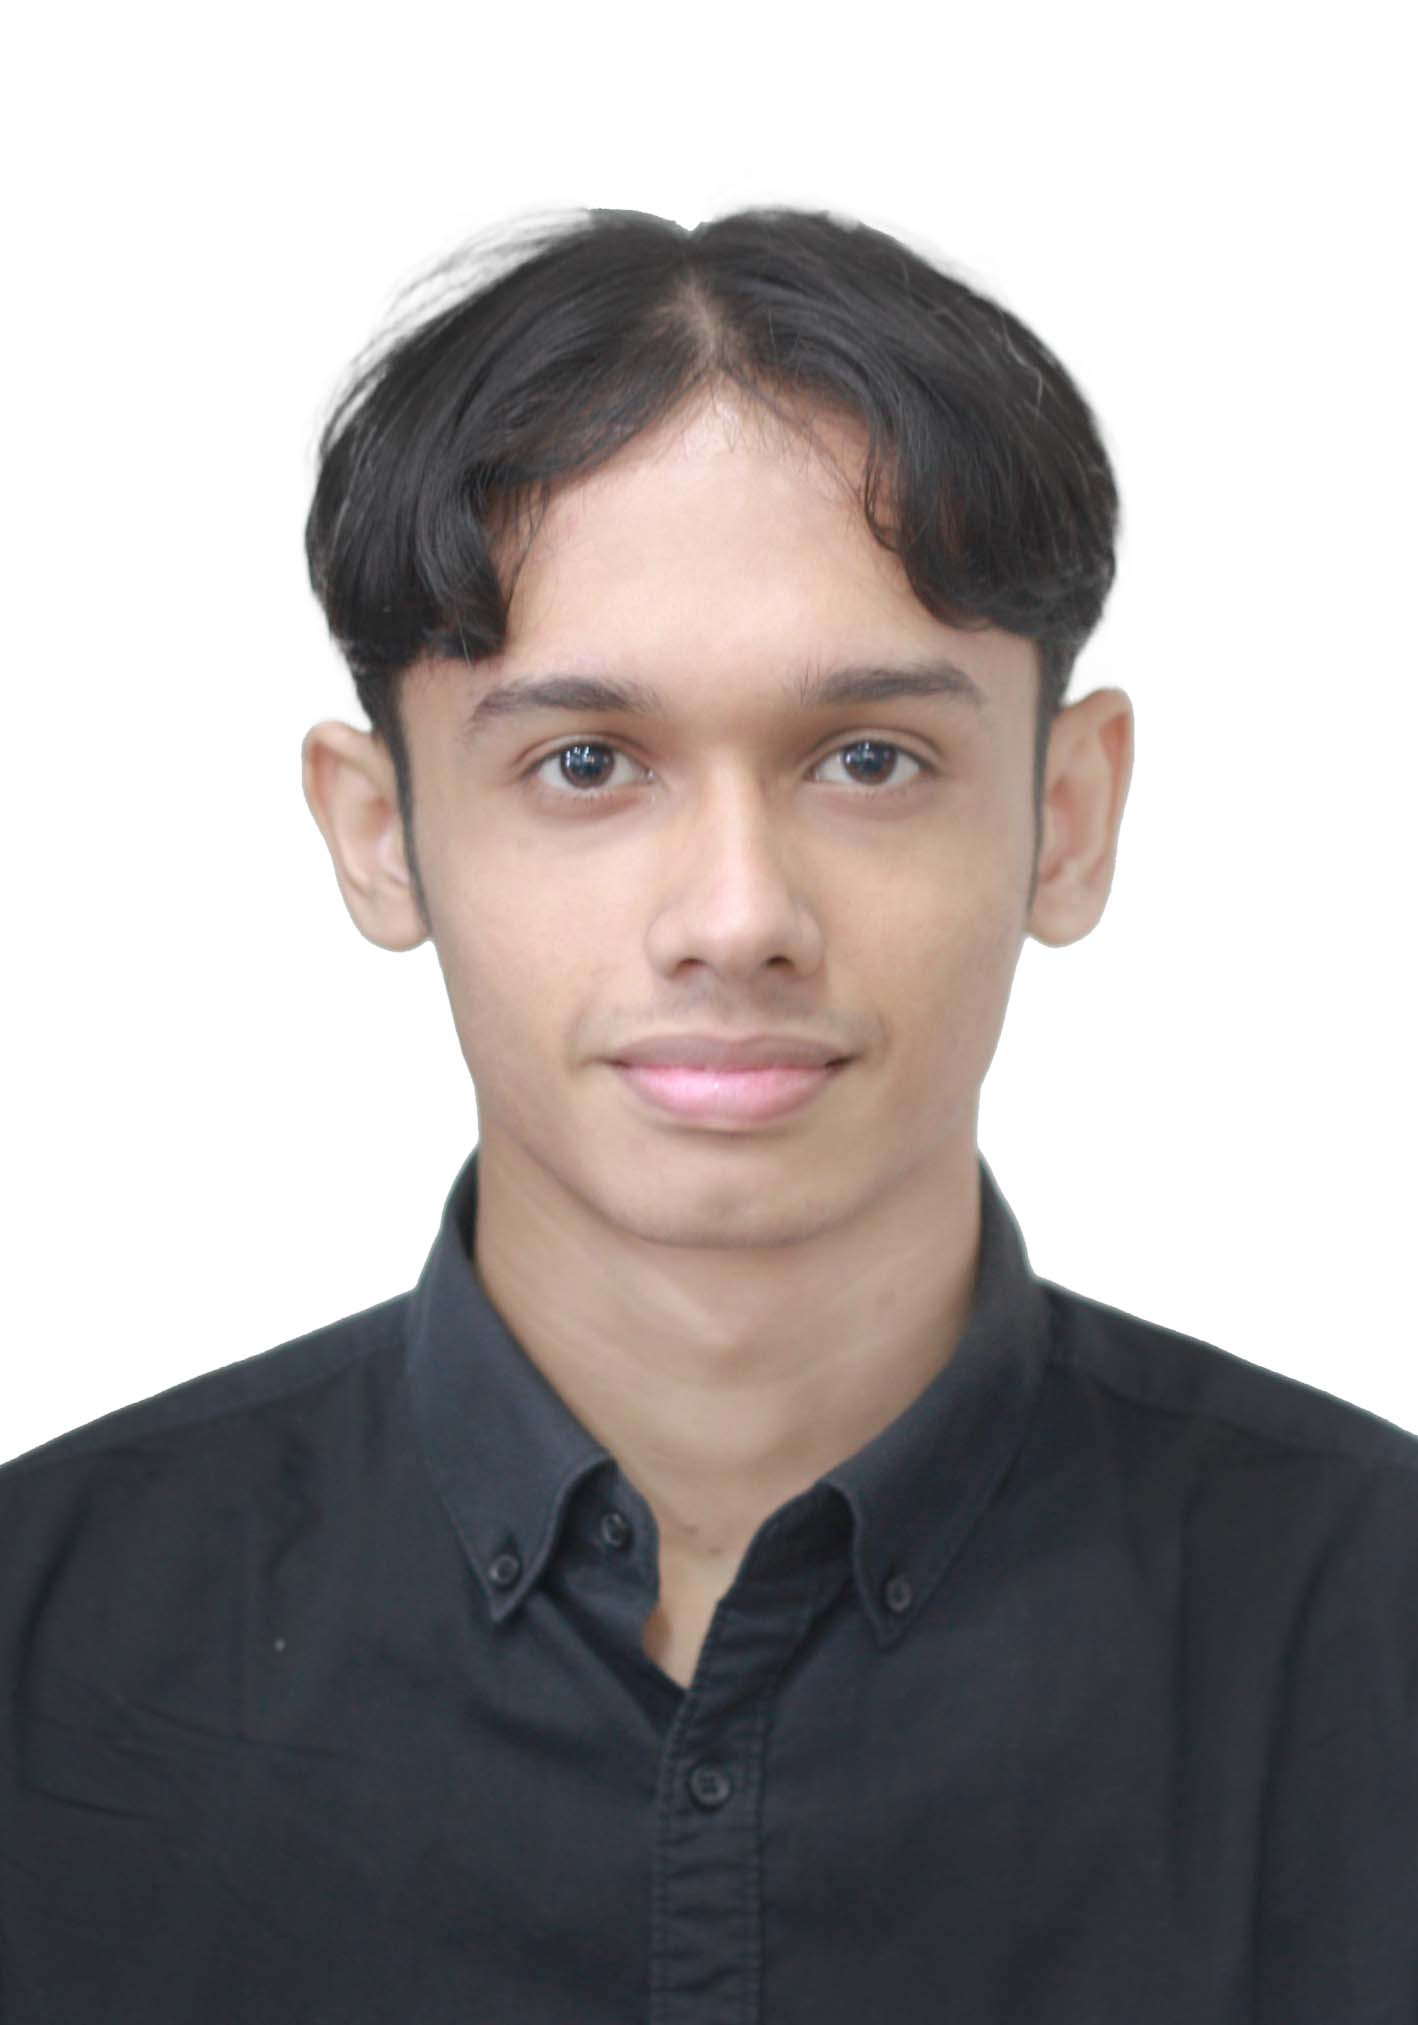
\includegraphics[width=2.0cm]{./profile-pic.jpg}
    \end{minipage}}  & {\textbf{\Large AZRYL SHAMIN BIN AZRIZAL}} & \\
  & {\textit{BSc in Computer Science | Software Engineering}} & {} \\
  & {} & {} \\
  & {\small Email: \textbf{\href{mailto:azryl.career@gmail.com}{azryl.career@gmail.com}}} & {\small GitHub: \textbf{\href{https://github.com/azrylshamin}{github.com/azrylshamin}}} \\
  & {\small Mobile: \textbf{\href{tel:+601110169553}{+6011-1016 9553}}} & {\small LinkedIn: \textbf{\href{https://www.linkedin.com/in/azrylshamin/}{linkedin.com/in/azrylshamin}}}\\
\end{tabular*}

%-----------ABOUT ME-----------------
\section{SKILLS}
\resumeSubHeadingListStart
\resumeSubItem{\textbf{Programming: }}{Javascript, Bash, Java, SQL, \CC, C\mytextsharp }
\resumeSubItem{\textbf{Front-End: }}{React, Next.js, HTML/CSS, Tailwind CSS}
\resumeSubItem{\textbf{Back-End: }}{Node.js, Express.js}
\resumeSubItem{\textbf{Databases: }}{PostgreSQL, MongoDB}
\resumeSubHeadingListEnd


%-----------Experience-----------------
\section{EXPERIENCE}
\resumeSubHeadingListStart

\resumeSubheading
{System Developer Intern}{July 2024 -- October 2024}
{Majlis Amanah Rakyat}{Kuala Lumpur, Malaysia}
\resumeItemListStart
\resumeItem{Developed a \textbf{computer purchase claim application system} for the staff members using Blazor and .NET}
{}
\resumeItem{Successfully adapted to new technologies (C\mytextsharp and .NET) to align with company standards and efficiently deliver a functional application.}
{}
\resumeItem{Led an intern team to archive hundreds of tender files, improving efficiency and quality control through a synchronized workflow.}
{}
\resumeItem{Facilitated hands-on training of the Microsoft Power Platform, building a low-code service request application with automated email notifications to enhance process visibility.}
{}
\resumeItemListEnd


\resumeSubHeadingListEnd

%-----------Education-----------------
\section{EDUCATION}
\resumeSubHeadingListStart
\resumeSubheading
{Multimedia University}{Cyberjaya, Malaysia}
{Bachelor of Computer Science (Honours) in Software Engineering}{Oct 2022 -- Oct 2026}
% \begin{spacing}{0.4}
%   \colorbox{yellow}{\it\footnotesize CGPA: 3.9744}
% \end{spacing}
\resumeSubSubheading{Foundation in Information Tehnology}{Aug 2021 -- Aug 2022}

\resumeSubHeadingListEnd

%-----------Projects-----------------
% \section{PROJECTS}
% \resumeSubHeadingListStart

% \resumeSubHeadingListEnd

%-----------ACADEMIA-----------------
% \section{ACADEMIA}
% \resumeSubHeadingListStart

% \resumeSubHeadingListEnd

%-----------Certifications-----------------
% \section{CERTIFICATIONS}
% \resumeSubHeadingListStart

% \resumeSubHeadingListEnd


%-----------Activities-----------------
\section{ACTIVITIES}

\resumeSubHeadingListStart

\resumeSubheading{Geco Asia - Break into AI: Hack to Hire Hackathon}{Nov 2025 - Dec 2025}
{2nd runner up}{TRX KL}
\resumeItemListStart
\resumeItem{}{Engineered a FastAPI and DynamoDB backend for an AI "Early-Warning System," converting lagging survey data into real-time burnout and attrition insights.}
\resumeItem{}{Developed an n8n and Gemini 2.0 pipeline to automate data cleaning and sentiment analysis, featuring custom normalization for local "Manglish" slang.}
\resumeItem{}{Designed a "Risk Engine" providing actionable HR interventions to reduce attrition and standardize engagement for 16,000+ employees.}
\resumeItemListEnd

\resumeSubheading{MMU HACK DAY 2025}{Aug 2025}
{1st runner up}{Multimedia University}
\resumeItemListStart
\resumeItem{}{Developed a CGPA tracking system using TypeScript and React with real-time calculations and semester-wise GPA monitoring}
\resumeItem{}{Implemented weighted assessment evaluation with 40\% formative and 60\% summative tracking and automated academic standing classification}
\resumeItem{}{Built analytical features including What-If calculators for grade projections and performance optimization with risk assessment}
\resumeItemListEnd

\resumeSubheading{UMHackathon 2025}{Apr 2025}
{Participant}{University of Malaya}

\resumeSubheading{Student College Committee}{Jan 2023 -- Jan 2025}
{Head of Division (Business Operation Division)}{Multimedia University}

\resumeSubheading{CodeNection 2022 (Competitive Programming)}{13th Nov 2022}
{Finalist}{Multimedia University}

\resumeSubHeadingListEnd


%-------------------------------------------
\end{document}

% -----Credits-----
% Template: Sourabh Bajaj
% License : MIT